\subsection{关于三角形的一些概念}\label{subsec:czjh1-3-1}

三角形是一种很简单但又是最常见的几何图形。
例如,大桥的钢梁,起重机的支架等,都是三角形结构(图 \ref{fig:czjh1-3-1})。
在小学已经学过一些三角形的初步知识,本章里,
我们将比较系统地研究三角形的许多重要性质以及它们的应用。

\begin{figure}[htbp]
    \centering
    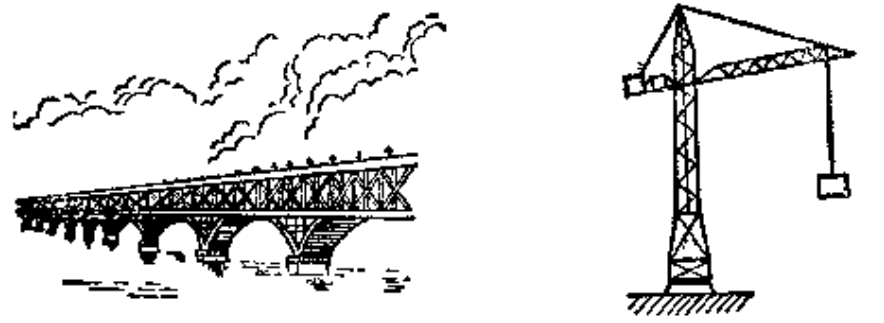
\includegraphics[width=12cm]{../pic/czjh1-ch3-01.png}
    \caption{}\label{fig:czjh1-3-1}
\end{figure}

如图 \ref{fig:czjh1-3-2}, 由三条线段首尾顺次连结所组成的图形叫做\zhongdian{三角形}。
组成三角形的三条线段叫做\zhongdian{三角形的边},相邻两边的公共端点叫做\zhongdian{三角形的顶点}。
例如,线段 $AB$、$BC$、$CA$ 是三角形的边,点 $A$、$B$、$C$ 是三角形的顶点。

\begin{figure}[htbp]
    \centering
    \begin{minipage}[b]{5cm}
        \centering
        \begin{tikzpicture}
    \tkzDefPoints{0/0/B, 3.5/0/C, 2.2/2/A}

    \tkzDrawPolygon(A,B,C)
    \tkzLabelPoints[above](A)
    \tkzLabelPoints[left](B)
    \tkzLabelPoints[right](C)
\end{tikzpicture}


        \caption{}\label{fig:czjh1-3-2}
    \end{minipage}
    \qquad
    \begin{minipage}[b]{4.5cm}
        \centering
        \begin{tikzpicture}
    \tkzDefPoints{0/0/B, 2/0/C, 1.4/1.4/A}
    \tkzDefPointOnLine[pos=1.5](C,A)  \tkzGetPoint{D}

    \tkzDrawLines[add=0.4 and 0.4, dashed](A,B  B,C  A,C)
    \tkzDrawPolygon(A,B,C)
    \tkzLabelPoints[right](A)
    \tkzLabelPoints[above left](B)
    \tkzLabelPoints[above right](C)
    \tkzLabelPoints[left](D)
\end{tikzpicture}


        \caption{}\label{fig:czjh1-3-3}
    \end{minipage}
    \qquad
    \begin{minipage}[b]{4.5cm}
        \centering
        \begin{tikzpicture}
    \tkzDefPoints{0/0/B, 3.5/0/C, 3.1/2/A}
    \tkzDefLine[bisector](B,A,C)  \tkzGetPoint{d}
    \tkzInterLL(A,d)(B,C)  \tkzGetPoint{D}
    \tkzDefMidPoint(B,C)  \tkzGetPoint{E}
    \tkzDefLine[altitude](B,A,C)  \tkzGetPoint{F}

    \tkzDrawPolygon(A,B,C)
    \tkzDrawSegments(A,D  A,E  A,F)
    \tkzMarkRightAngle[size=0.2](A,F,B)
    \tkzLabelPoints[above](A)
    \tkzLabelPoints[right](C)
    \tkzLabelPoints[below](B,D)
    \tkzLabelPoints[below,xshift=-0.5em](E)
    \tkzLabelPoints[below,xshift=-0.3em](F)
\end{tikzpicture}


        \caption{}\label{fig:czjh1-3-4}
    \end{minipage}
\end{figure}

“三角形” 可以用符号 “$\triangle$” 表示,顶点是 $A$、$B$、$C$ 的三角形,
记作 “$\triangle ABC$”, 读作 “三角形 $ABC$”。

三角形相邻两边组成的角叫做\zhongdian{三角形的内角},简称\zhongdian{三角形的角}。
三角形的角的一边与另一边的反向延长线组成的角叫做\zhongdian{三角形的外角}。
例如在图 \ref{fig:czjh1-3-3} 中, $\angle BAC$ 是 $\triangle ABC$ 的一个内角,$\angle BAD$ 是一个外角。
三角形的外角也就是与它有公共顶点的内角的邻补角。

三角形一个角的平分线和这个角的对边相交,这个角的顶点和交点之间的线段叫做\zhongdian{三角形的角平分线}。
连结三角形一个顶点和它的对边中点的线段叫做\zhongdian{三角形的中线}。
三角形一个顶点到它的对边所在直线的垂线段叫做\zhongdian{三角形的高}。
在图 \ref{fig:czjh1-3-4} 中, 线段 $AD$ 是 $\triangle ABC$ 的角平分线, $AE$ 是中线, $AF$ 是高。

\begin{figure}[htbp]
    \centering
    \begin{minipage}[b]{7cm}
        \centering
        \begin{tikzpicture}
    \tkzDefPoints{0/0/B, 3.5/0/C, 2.8/2/A}
    \tkzDefLine[bisector](B,A,C) \tkzGetPoint{d}
    \tkzDefLine[bisector](A,B,C) \tkzGetPoint{e}
    \tkzDefLine[bisector](B,C,A) \tkzGetPoint{f}
    \tkzInterLL(A,d)(B,C)        \tkzGetPoint{D}
    \tkzInterLL(B,e)(A,C)        \tkzGetPoint{E}
    \tkzInterLL(C,f)(A,B)        \tkzGetPoint{F}

    \tkzDrawPolygon(A,B,C)
    \tkzDrawSegments(A,D  B,E  C,F)
    \tkzMarkAngle[size=0.5](E,B,A)
    \tkzMarkAngle[size=0.6](C,B,E)
    \tkzMarkAngle[size=0.5, arc=ll](F,C,B)
    \tkzMarkAngle[size=0.6, arc=ll](A,C,F)
    \tkzMarkAngle[size=0.5, arc=lll](B,A,D)
    \tkzMarkAngle[size=0.6, arc=lll](D,A,C)
    \tkzLabelPoints[above](A)
    \tkzLabelPoints[left](B,F)
    \tkzLabelPoints[right](C,E)
    \tkzLabelPoints[below](D)
\end{tikzpicture}


        \caption*{甲}
    \end{minipage}
    \qquad
    \begin{minipage}[b]{7cm}
        \centering
        \begin{tikzpicture}
    \tkzDefPoints{0/0/B, 3.5/0/C, 2.8/2/A}
    \tkzDefMidPoint(B,C)  \tkzGetPoint{D}
    \tkzDefMidPoint(A,C)  \tkzGetPoint{E}
    \tkzDefMidPoint(A,B)  \tkzGetPoint{F}

    \tkzDrawPolygon(A,B,C)
    \tkzDrawSegments(A,D  B,E  C,F)
    \tkzMarkSegments[mark=|](B,D  D,C)
    \tkzMarkSegments[mark=||](A,E  E,C)
    \tkzMarkSegments[mark=|||](A,F  F,B)
    \tkzLabelPoints[above](A)
    \tkzLabelPoints[left](B,F)
    \tkzLabelPoints[right](C,E)
    \tkzLabelPoints[below](D)
\end{tikzpicture}


        \caption*{乙}
    \end{minipage}
    \caption{}\label{fig:czjh1-3-5}
\end{figure}

三角形有三条角平分线(图 \ref{fig:czjh1-3-5} 甲), 三条中线(图 \ref{fig:czjh1-3-5} 乙)。
它们都在三角形的内部。

三角形也有三条高。 由于三角形的内角可能是锐角也可能是钝角或直角,三角形的高不一定都在三角形内部。
如图 \ref{fig:czjh1-3-6} , 图甲中三条高都在三角形内部;
图乙中有一条在三角形内部,另外两条在三角形外部;
图丙中有一条在三角形内部,而另外两条恰好是三角形的两条边。

\begin{figure}[htbp]
    \centering
    \begin{minipage}[b]{4.5cm}
        \centering
        \begin{tikzpicture}
    \tkzDefPoints{0/0/B, 3/0/C, 2.4/2/A}
    \tkzDefLine[altitude](B,A,C)  \tkzGetPoint{D}
    \tkzDefLine[altitude](C,B,A)  \tkzGetPoint{E}
    \tkzDefLine[altitude](A,C,B)  \tkzGetPoint{F}

    \tkzDrawPolygon(A,B,C)
    \tkzDrawSegments(A,D  B,E  C,F)
    \tkzMarkRightAngle[size=0.15](A,D,C)
    \tkzMarkRightAngle[size=0.15](B,E,A)
    \tkzMarkRightAngle[size=0.15](C,F,B)
    \tkzLabelPoints[above](A)
    \tkzLabelPoints[left](B,F)
    \tkzLabelPoints[right](C,E)
    \tkzLabelPoints[below](D)
\end{tikzpicture}


        \caption*{甲}
    \end{minipage}
    \qquad
    \begin{minipage}[b]{4cm}
        \centering
        \begin{tikzpicture}
    \tkzDefPoints{0/0/B, 1/0/C, 2.4/2/A}
    \tkzDefLine[altitude](B,A,C)  \tkzGetPoint{D}
    \tkzDefLine[altitude](C,B,A)  \tkzGetPoint{E}
    \tkzDefLine[altitude](A,C,B)  \tkzGetPoint{F}

    \tkzDrawPolygon(A,B,C)
    \tkzDrawSegments(A,D  B,E  C,F)
    \tkzDrawSegments[dashed](C,D  C,E)
    \tkzMarkRightAngle[size=0.15](A,D,C)
    \tkzMarkRightAngle[size=0.15](B,E,A)
    \tkzMarkRightAngle[size=0.15](C,F,B)
    \tkzLabelPoints[above](A)
    \tkzLabelPoints[left](B,F)
    \tkzLabelPoints[below, xshift=0.5em](C)
    \tkzLabelPoints[below](D,E)
\end{tikzpicture}


        \caption*{乙}
    \end{minipage}
    \begin{minipage}[b]{5.0cm}
        \centering
        \begin{tikzpicture}
    \tkzDefPoints{0/0/B, 3/0/C, 3/2/A}
    \tkzDefLine[altitude](A,C,B)  \tkzGetPoint{F}

    \tkzDrawPolygon(A,B,C)
    \tkzDrawSegments(C,F)
    \tkzMarkRightAngle[size=0.15](A,C,B)
    \tkzMarkRightAngle[size=0.15](C,F,B)
    \tkzLabelPoints[above](A)
    \tkzLabelPoints[below](B)
    \tkzLabelPoints[left](F)
    \tkzLabelPoints[right](C)
\end{tikzpicture}


        \caption*{丙}
    \end{minipage}
    \caption{}\label{fig:czjh1-3-6}
\end{figure}


\begin{lianxi}

\xiaoti{}%
\begin{xiaoxiaotis}%
    \xxt[\xxtsep]{说出图中有几个三角形,把它们读出来。 说明 $\angle ACD$ 是哪个三角形的内角,哪个三角形的外角;}

    \xxt{写出在 $\triangle ABD$ 中, $\angle B$ 所对的边、边 $BD$ 所对的角。}

\end{xiaoxiaotis}


\begin{figure}[htbp]
    \centering
    \begin{minipage}[b]{4.5cm}
        \centering
        \begin{tikzpicture}
    \tkzDefPoints{0/0/B, 3.5/0/E, 1.8/2/A,  0.8/0/C, 2.8/0/D}

    \tkzDrawPolygon(A,B,E)
    \tkzDrawSegments(A,C  A,D)
    \tkzLabelPoints[above](A)
    \tkzLabelPoints[below](B,C,D,E)
\end{tikzpicture}


        \caption*{(第 1 题)}
    \end{minipage}
    \qquad
    \begin{minipage}[b]{4.5cm}
        \centering
        \begin{tikzpicture}
    \tkzDefPoints{0/0/B, 3.5/0/C, 3.1/2/A}
    \tkzDefLine[bisector](B,A,C)  \tkzGetPoint{d}
    \tkzInterLL(A,d)(B,C)  \tkzGetPoint{D}
    \tkzDefMidPoint(B,C)  \tkzGetPoint{E}
    \tkzDefLine[altitude](B,A,C)  \tkzGetPoint{F}

    \tkzDrawPolygon(A,B,C)
    \tkzDrawSegments(A,D  A,E  A,F)
    \tkzMarkRightAngle[size=0.2](A,F,B)
    \tkzLabelPoints[above](A)
    \tkzLabelPoints[right](C)
    \tkzLabelPoints[below](B,D)
    \tkzLabelPoints[below,xshift=-0.5em](E)
    \tkzLabelPoints[below,xshift=-0.3em](F)
\end{tikzpicture}


        \caption*{(第 2 题)}
    \end{minipage}
    \qquad
    \begin{minipage}[b]{4.5cm}
        \centering
        \begin{tikzpicture}
    \tkzDefPoints{0/0/B, 3.4/0/C, 1.7/2/A, 1.7/0/D}

    \tkzDrawPolygon(A,B,C)
    \tkzDrawSegments(A,D)
    \tkzMarkRightAngle(A,D,B)
    \tkzLabelPoints[above](A)
    \tkzLabelPoints[below](B,C,D)
\end{tikzpicture}


        \caption*{(第 3 题)}
    \end{minipage}
\end{figure}

\begin{enhancedline}
\xiaoti{如图,在 $\triangle ABC$ 中, 已知 $AE$ 是中线, $AD$ 是角平分线,$AF$ 是高。根据已知条件填空:}
\begin{xiaoxiaotis}

    \xxt{$BE = \ewkh[1cm] = \exdfrac{1}{2} \ewkh[1cm]$;}

    \xxt{$\angle BAD = \ewkh[1cm] = \exdfrac{1}{2} \ewkh[1cm]$;}

    \xxt{$\angle AFB = \ewkh[1cm] = Rt \angle$。}

\end{xiaoxiaotis}
\end{enhancedline}


\xiaoti{如图,$AD$ 同时是 $\triangle ABC$ 的高、中线和角平分线。 在括号内填写下列等式的根据:}
\begin{xiaoxiaotis}

    \xxt{$\angle ADB = \angle ADC$(\hspace*{2cm});}

    \xxt{$\angle DAB = \angle DAC$(\hspace*{2cm});}

    \xxt{$BD = DC$(\hspace*{2cm})。}

\end{xiaoxiaotis}

\end{lianxi}


